\chapter{DESIGN DETAILS AND IMPLEMENTATION}
Data collection is major and the most tedious part of this project because we required the data from specific geolocation and time duration. For our thesis we have collected data from twitter in JSON format and later converted into CSV file . We are going to describe how data is fetched , stored ,cleaned, processed and classified. Before exploring these processes ,let us explain our proposed architecture.
\section{Proposed Architecture}
Our goal is to examine degree of concern regarding 'Zika virus' by analyzing sentiment polarity of tweets. We  are going to pursue following steps to achieve our objective.\\
\begin{figure}[h]
\label{11dr1}
\centerline{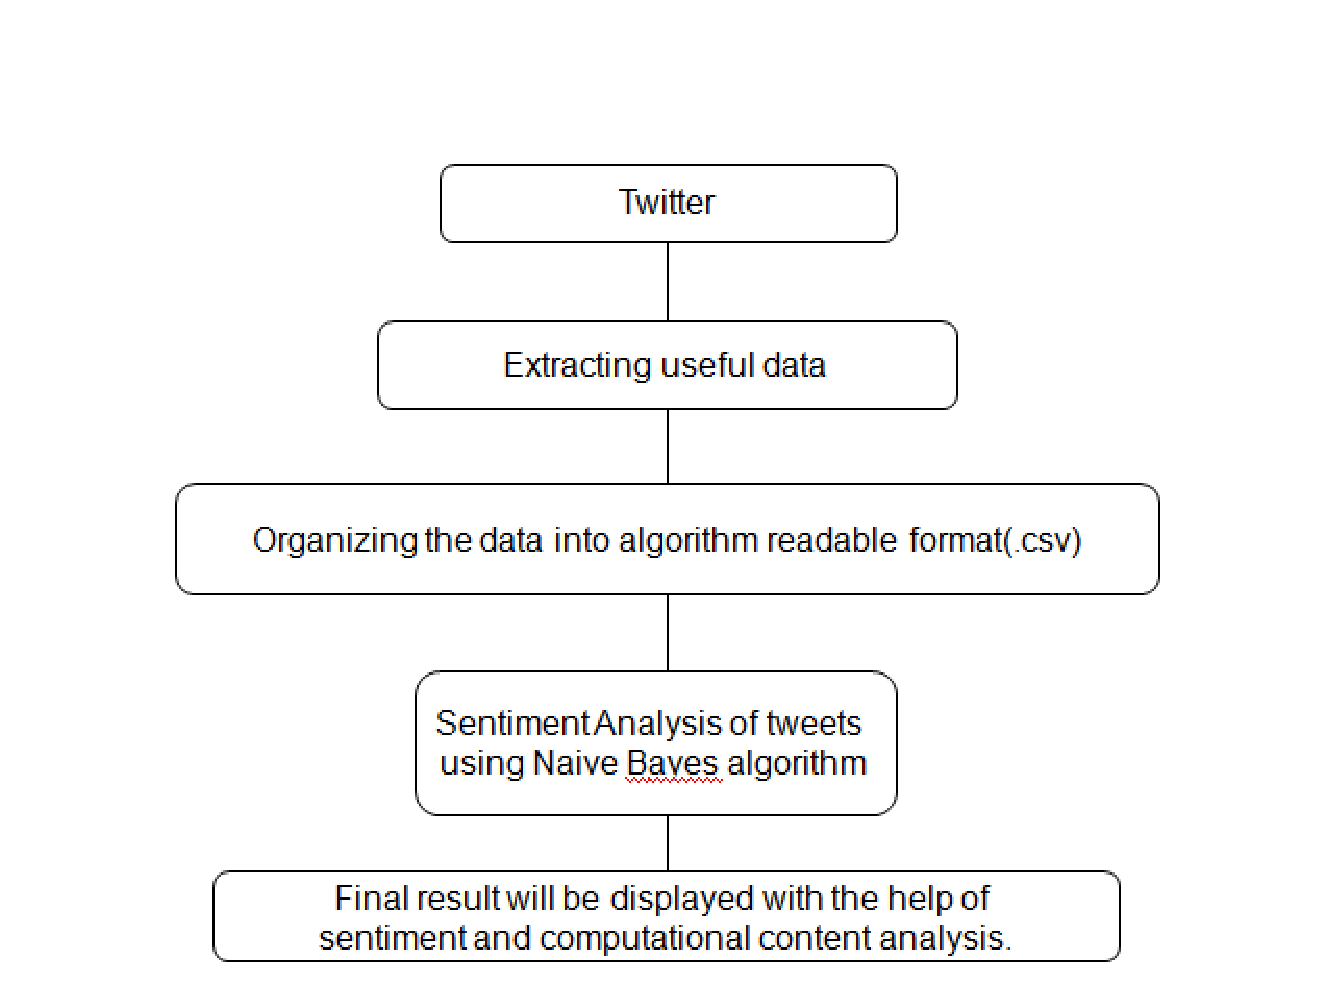
\includegraphics[width=4in]{11dr1}}
\caption{Flowchart of proposed activities}
\end{figure}\\
{\bf Step1 :}We are going to extract raw tweets from twitter by using tweepy libraries in python.\\
{\bf Step2 :}Then we clean these tweets and remove repeated tweets so that they can be fit for the desired  Sentiment analysis algorithm.\\
{\bf Step3 :}After preprocessing the data we are going to use this data set in the algorithm which will classify them as per their polarity .\\
{\bf Step4 :}Then we are going to calculate the degree of concern regarding 'Zika virus'.\\
Since, We are going to collect data from twitter so we are going to use twitter application for this purpose.
 The steps are shown in flowchart given in figure \ref{11dr1}.
\section{Twitter API}
Twitter API is used to extract tweets from twitter. There are two types of twitter APIs : Streaming API and REST API.
\subsection{Streaming API}
Streaming API is used to collect real time tweets .
\subsection{REST API}
Limited data can be fetched using REST API.
\section{Data Collection}
\subsection{Twitter data}
We need a twitter account for using Twitter API .A twitter account can be easily created by filling a sign up form on twitter. Now you will get your login credentials which is used to create our API. We are provided customer secret key, consumer key , access token key and access secret key. These keys are used for authentication purpose while extracting data from twitter.
\par Since the objective of this thesis is to examine degree of concern regarding 'Zika virus' by analyzing sentiment polarity of tweets from specific geolocation  so we need tweets which contains keywords 'zika' ,'zika virus' .We have created  python script for fetching tweets from  twitter with keywords 'zika' ,'zika virus' .Before creating this script we required to install Python library known as  {\bf tweepy}.
\par Tweepy is the Python library which helps us to communicate with twitter and use its API to  extract data which further can be used in the algorithm to determine sentiment polarity of tweets. Tweepy can be installed by simply using command 'pip install tweepy' in command prompt.
In this python script we used  customer secret key, consumer key , access token key and access secret key which we are provided with API. First we create function that loads the twitter API after authorizing the user .
\par We have used following functions in our Python script:\\

   {\bf 1. load_api :} This function loads the twitter API after authorizing the user. In this we use OAth protocol which authorizes the user. OAth provide security and authontication to user.
   {\bf 2. tweet_search :} This function consists of a search string 'query' , max_tweets ,minimum_tweet id , geocode and since id .
 {\bf 3. get_tweet_id :}  We use get_tweet_id function in order to get the ID which is considered as 'staring point'
  {\bf 4. write_tweets :} This function writes tweets to a file in JSON format .
  {\bf 5. main() :} This script continuously searches for tweets . In this part of the script we can input the specific duration (maximum 9 days old) as well as specific phrase(Zika in this thesis ) which we want in fetched  tweets.




\begin{figure}[h]
\centerline{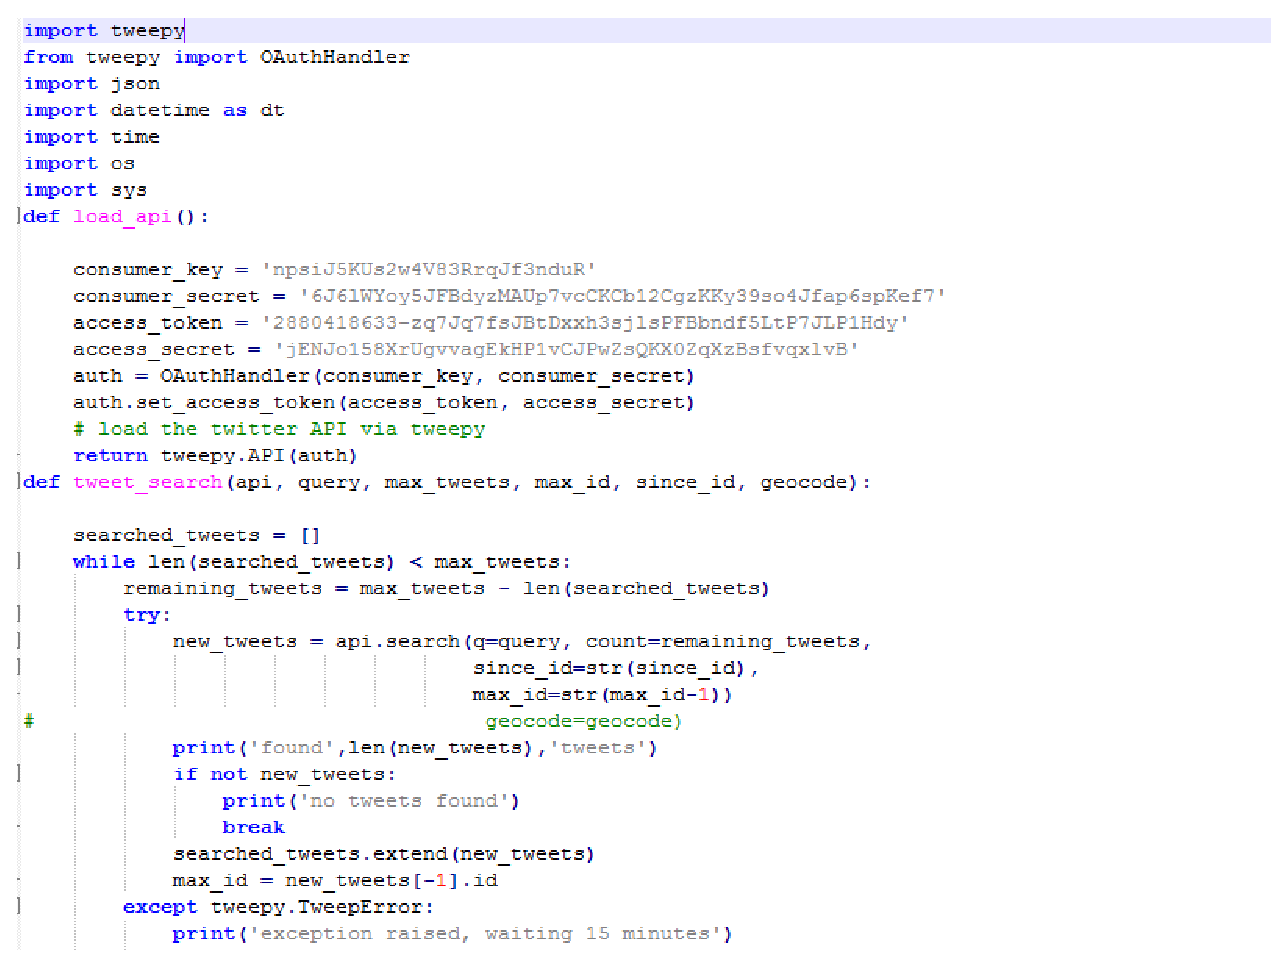
\includegraphics[width=5.7in]{CODE-0}}
\caption{Python code for extracting tweets}
\end{figure}
\begin{figure}[h]
\centerline{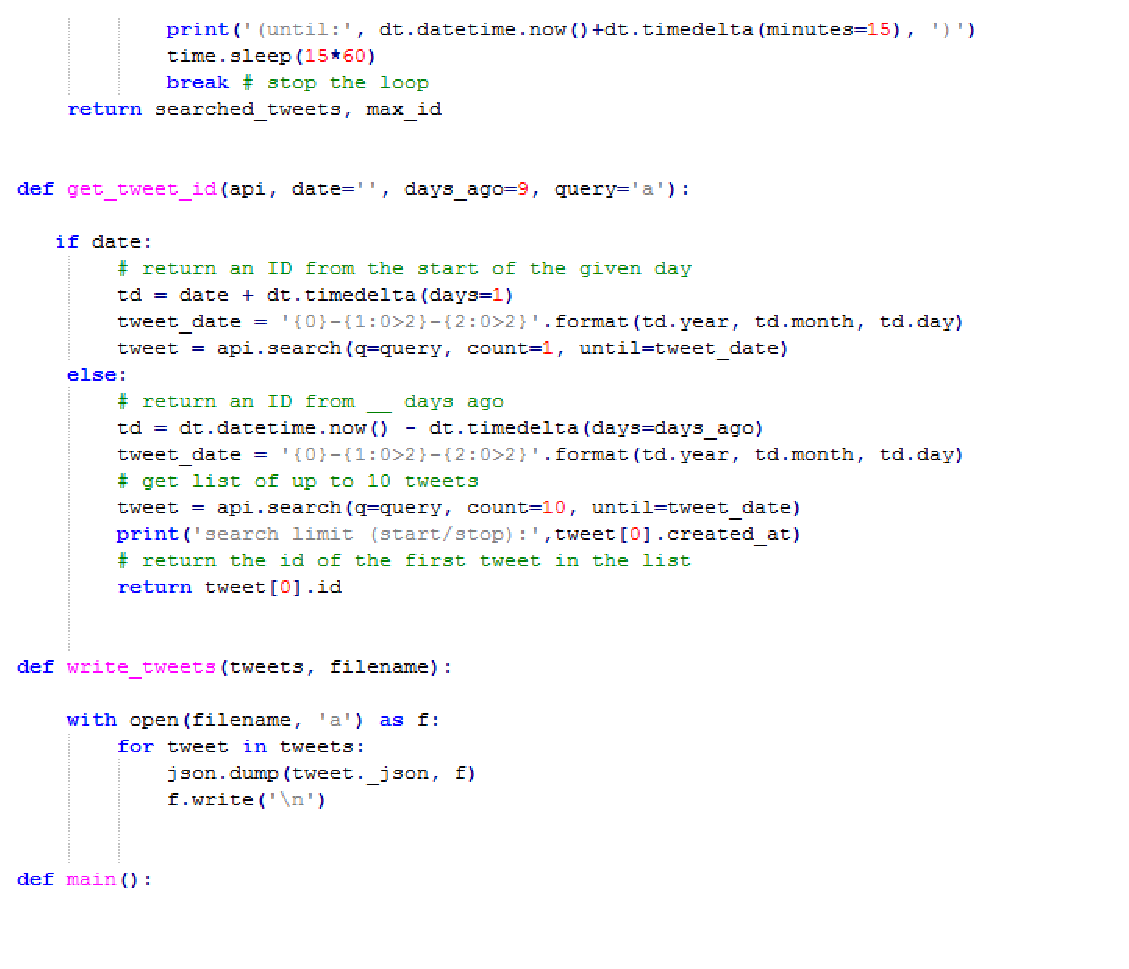
\includegraphics[width=5.7in]{CODE-1}}
\caption{Python code for extracting tweets}
\end{figure}
\begin{figure}[h]
\centerline{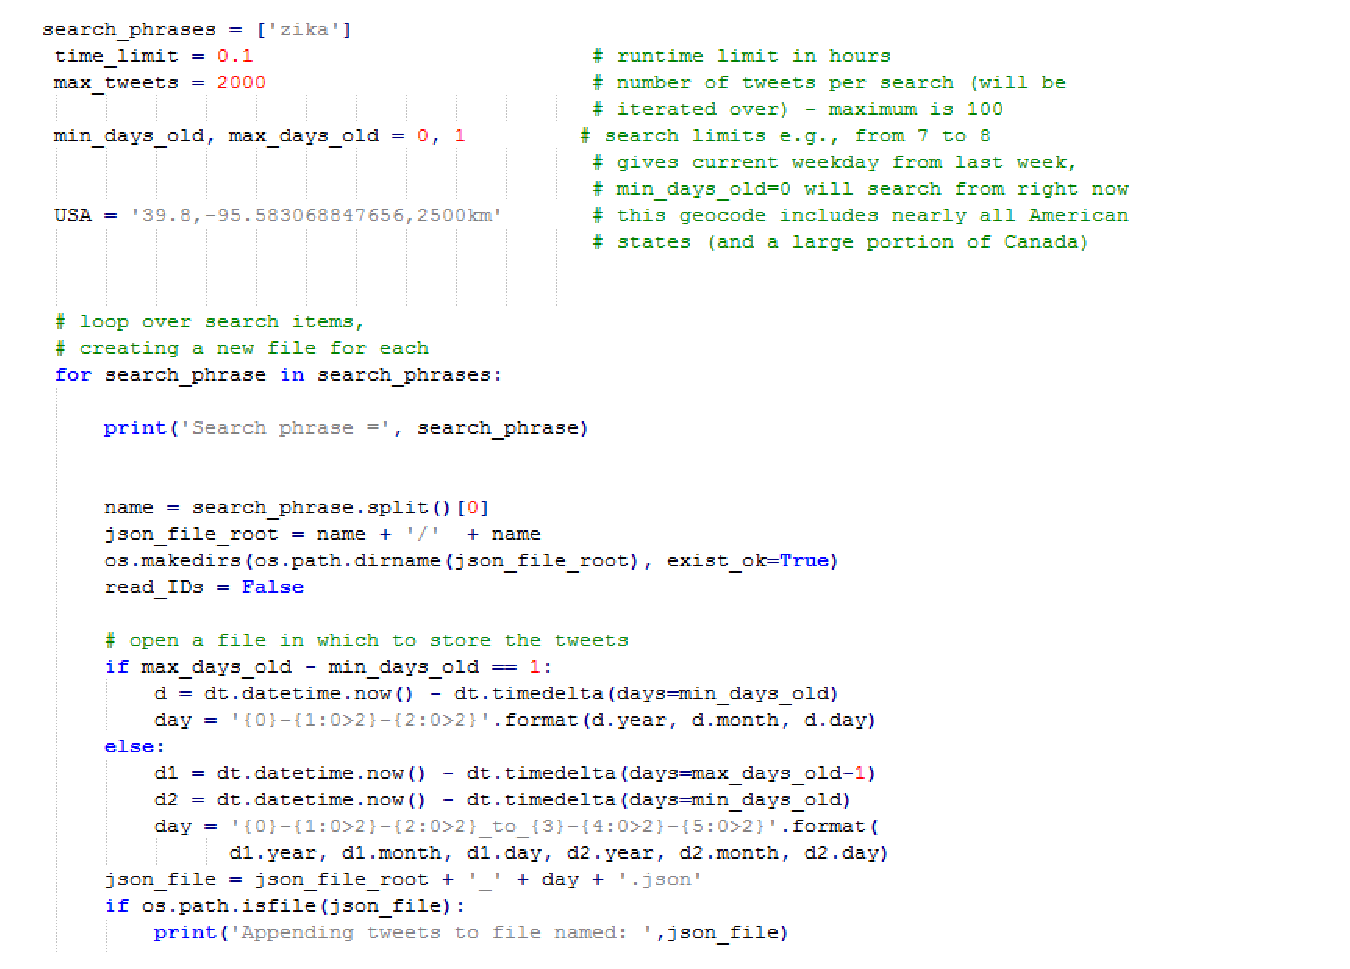
\includegraphics[width=5.7in]{CODE-2}}
\caption{Python code for extracting tweets}
\end{figure}
\begin{figure}[h]
\centerline{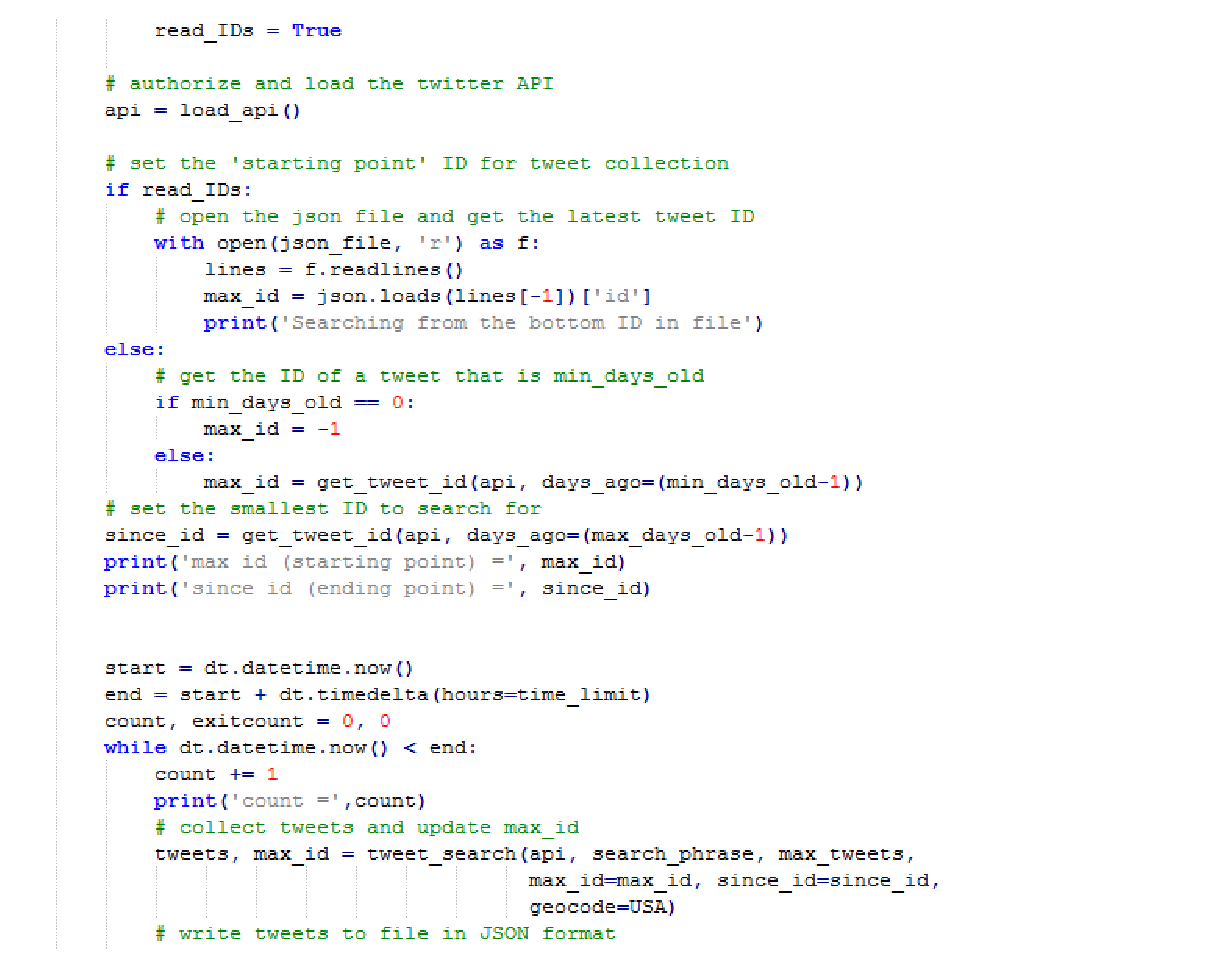
\includegraphics[width=5.7in]{CODE-3}}
\caption{Python code for extracting tweets}
\end{figure}
\begin{figure}[h]
\centerline{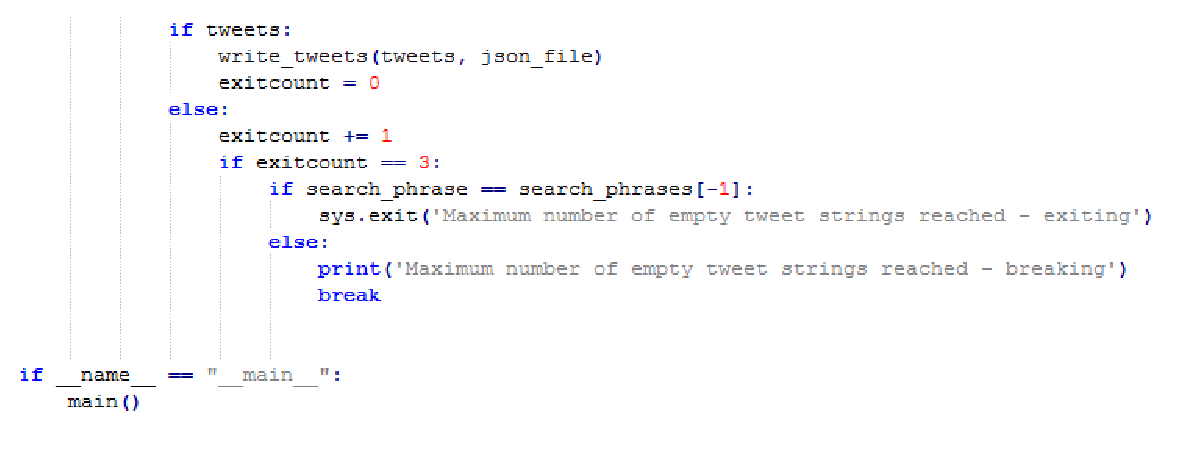
\includegraphics[width=5.7in]{CODE-4}}
\caption{Python code for extracting tweets}
\end{figure}

\section{Data Storage}
      Once , we start extracting tweets by using Twitter API we required to store that dataset  as a algorithm readable format . We stored 26,239 tweets from 30 July , 2017 to 6 August having keywords 'Zika' and  ' Zika Virus '  . Everytime a JSON (JavaScript Object Notation)  is generated when we ran our python script . These JSON files consist of raw tweets with other informations regarding all the particular tweets such as the date when the tweet is done , retweets  , geolocation and other informations. Since the CSV(Comma Seperated Value) format is easily  accessible , we converted the JSON dataset into CSV format . CSV files can be written/read in less time compared to other formats.
 \begin{figure}[h]
\centerline{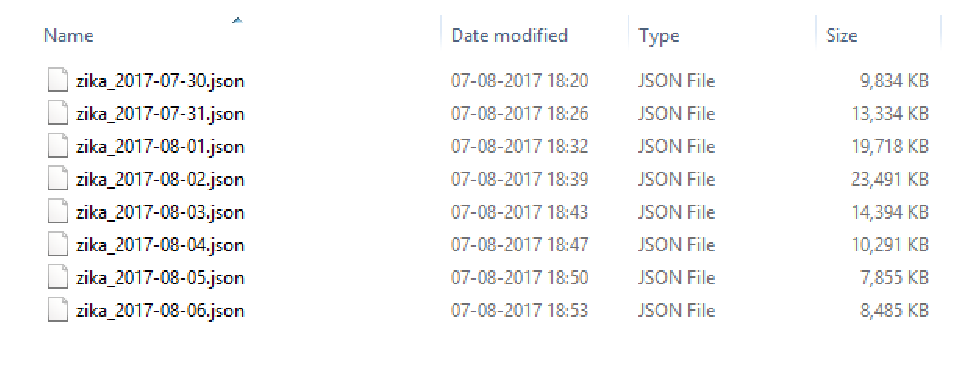
\includegraphics[width=5.7in]{tw1}}
\caption{.json files containing tweets}
\end{figure}


We stored tweets from different dates in different directories in the computer hard drive . Then we required to pre-process  and clean the data before using it on algorithm for finding out sentiment polarity . So in our next step we pre-processed  the data .
\section{Data Preprocessing}
    Data obtained from twitter consists of a lot of other information along with tweets which is not fit for extracting features. The raw tweets consist of message along with its metadata .\\
     We required only  tweet text to implement it on our algorithm so we removed all  other metadata such as creation date , language code , location and other informations .\\
    Following figures are of  one sample raw tweet and its text message .
 \begin{figure}[h]
\centerline{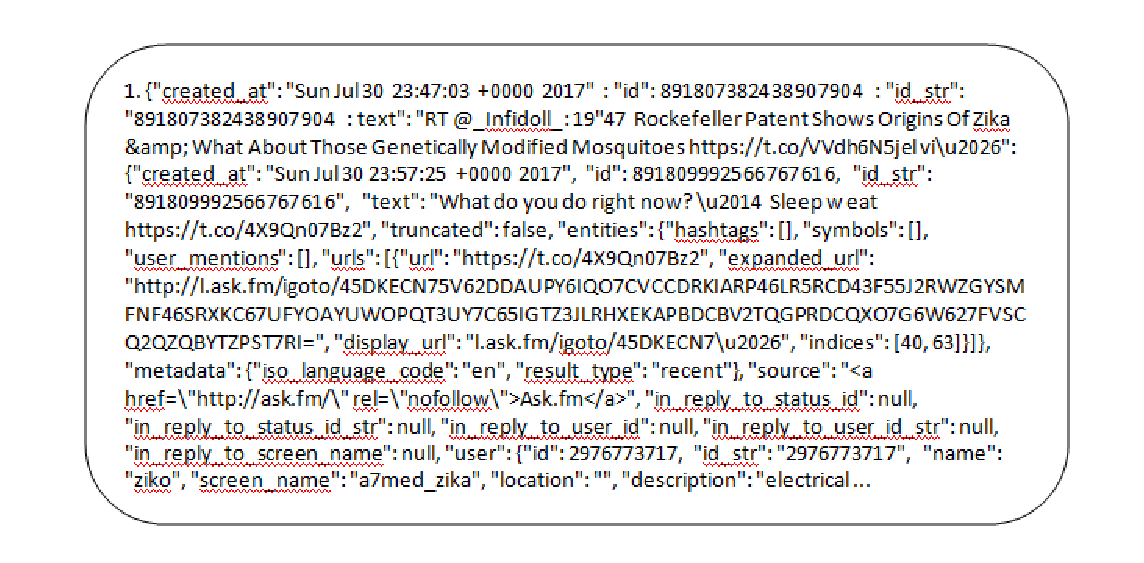
\includegraphics[width=5.7in]{ort}}
\caption{Sample of one raw tweet}
\end{figure}
  \begin{figure}[h]
\centerline{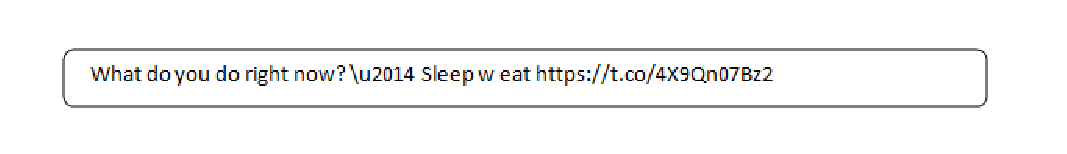
\includegraphics[width=5.7in]{oct}}
\caption{Text message of the tweet}
\end{figure}
We removed all the stop words ( like is , this ,the , he , a etc. ) from the  main message of the tweet  by using various NLTK functions .\\
After pre-processing the data it is ready for our next step which is to use this pre-processed dataset  on algorithm  to classify them into different polarity groups (positive, negative, neutral ).
\section{Classification}
Sentiment analysis or opinion mining is the process through which we decide any write up in to three polarity classes which are positive , negative and neutral .For classifying the tweets into different polarity  classes there are many techniques and algorithm available  . So we classified the tweets in different classes (positive, negative , neutral)  by using one of the techniques 'Naive - Bayes Classifier' .
\begin{figure}[h]
\centerline{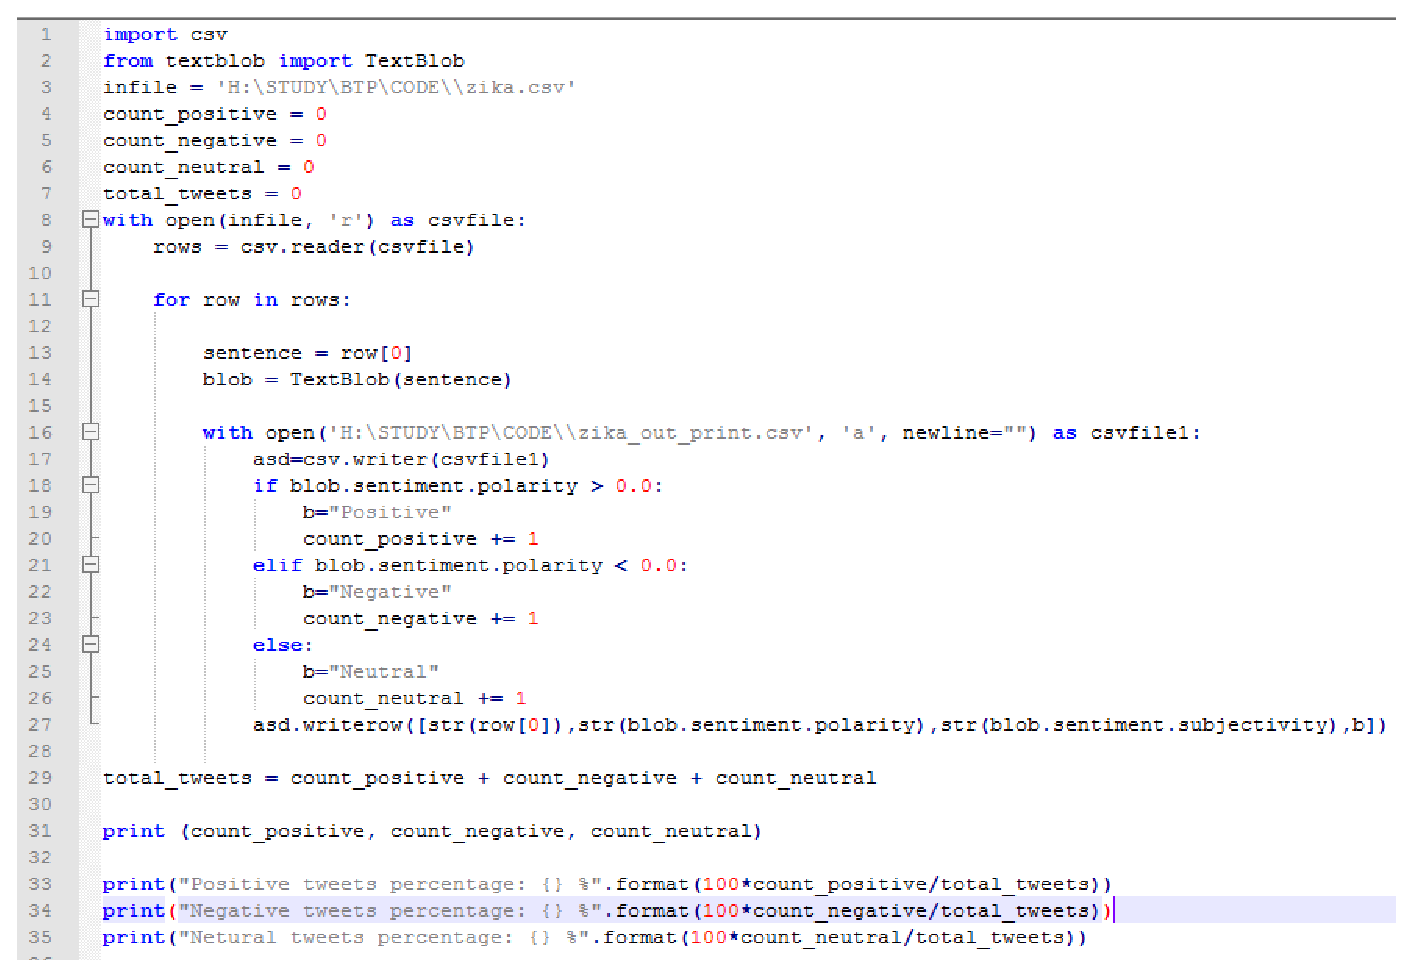
\includegraphics[width=5.7in]{sac}}
\caption{Code for sentiment analysis}
\end{figure}

